\documentclass[%
 reprint,
%superscriptaddress,
%groupedaddress,
%unsortedaddress,
%runinaddress,
%frontmatterverbose, 
%preprint,
%showpacs,preprintnumbers,
%nofootinbib,
%nobibnotes,
%bibnotes,
 amsmath,amssymb,
 aps,
%pra,
%prb,
%rmp,
%prstab,
%prstper,
%floatfix,
nobalancelastpage
]{revtex4-1}

\usepackage{graphicx}
\usepackage{dcolumn}
\usepackage{bm}
\usepackage{chemformula}
\usepackage{gensymb} 

\setlength{\parskip}{1em}

\begin{document}
\title{Cell staining protocol for intranuclear staining of A673 U2\#83 with sticky batches of PA-JF646}
\author{Shawn Yoshida$^{1,2}$, Shasha Chong$^{1}$ \\
        \small $^{1}$Division of Chemistry and Chemical Engineering, California Institute of Technology, Pasadena, CA, USA \\
        \small $^{2}$Division of Biology and Biological Engineering, California Institute of Technology, Pasadena, CA, USA
}

\date{9/29/2021}

\maketitle



\section{\label{sec:level1}Introduction}

A common issue with the staining of intranuclear targets with photoactivatable (PA) Janelia Fluor\textsuperscript{\textregistered} dyes such as PA-JF646 is the non-specific binding of HaloTag\textsuperscript{\textregistered} ligands to cytoplasmic junk. By supplementing the growth media with additional fetal bovine serum (FBS) and extending post-staining washing times as described below, the FBS out-competes much of the PA-JF646 non-specific, cytoplasmic binding.

\,

\section{\label{sec:level2}Staining protocol}

FBS-boosted growth media composition: 
20\% FBS, 1\% Penicillin Streptomycin (pen-strep) 
\begin{enumerate}
  \item Make a 200nM dilution of PA-JF646 in the FBS-boosted growth media. 
  \item Asprirate old growth media, then rinse cells twice with 1X phosphate-buffered saline (PBS).
  \item Incubate cells with the HaloTag\textsuperscript{\textregistered} ligand-containing media at 37\degree C for 15 minutes. 
  \item Asprirate HaloTag\textsuperscript{\textregistered} ligand-containing media, then rinse cells twice with 1X phosphate-buffered saline (PBS). 
  \item Incubate with FBS-boosted media (without ligands) for 1 hour, then rinse cells twice with 1X phosphate-buffered saline (PBS). Repeat this whole step twice. 
\end{enumerate}

The cells should be ready to image or fix at this point.

\section{\label{sec:level3}Notes:}

Aliquots of HaloTag\textsuperscript{\textregistered} ligands can be kept in the -80\degree C or -20\degree C. Do be especially careful when handling them. 

\begin{itemize}
  \item Fully thaw aliquot before opening to prevent contamination via condensation
  \item Minimize exposure of fluorophores to light. 
  \item Minimize the amount of time the aliquot of fluorophores is out of the freezer. 
\end{itemize}

When the modified staining protocol is used (even with sticky batches of PA-JF646), a majority of the signal is localized to the nucleus (\ref{fig1}). While we typically face fewer issues with lower wavelength dyes like PA-JF549, depending on the batch, we still often see some amount of unwanted fluorescent signal from the cytoplasm. This can be nearly entirely eliminated with this protocol (\ref{fig2}).

\begin{figure}[b] 
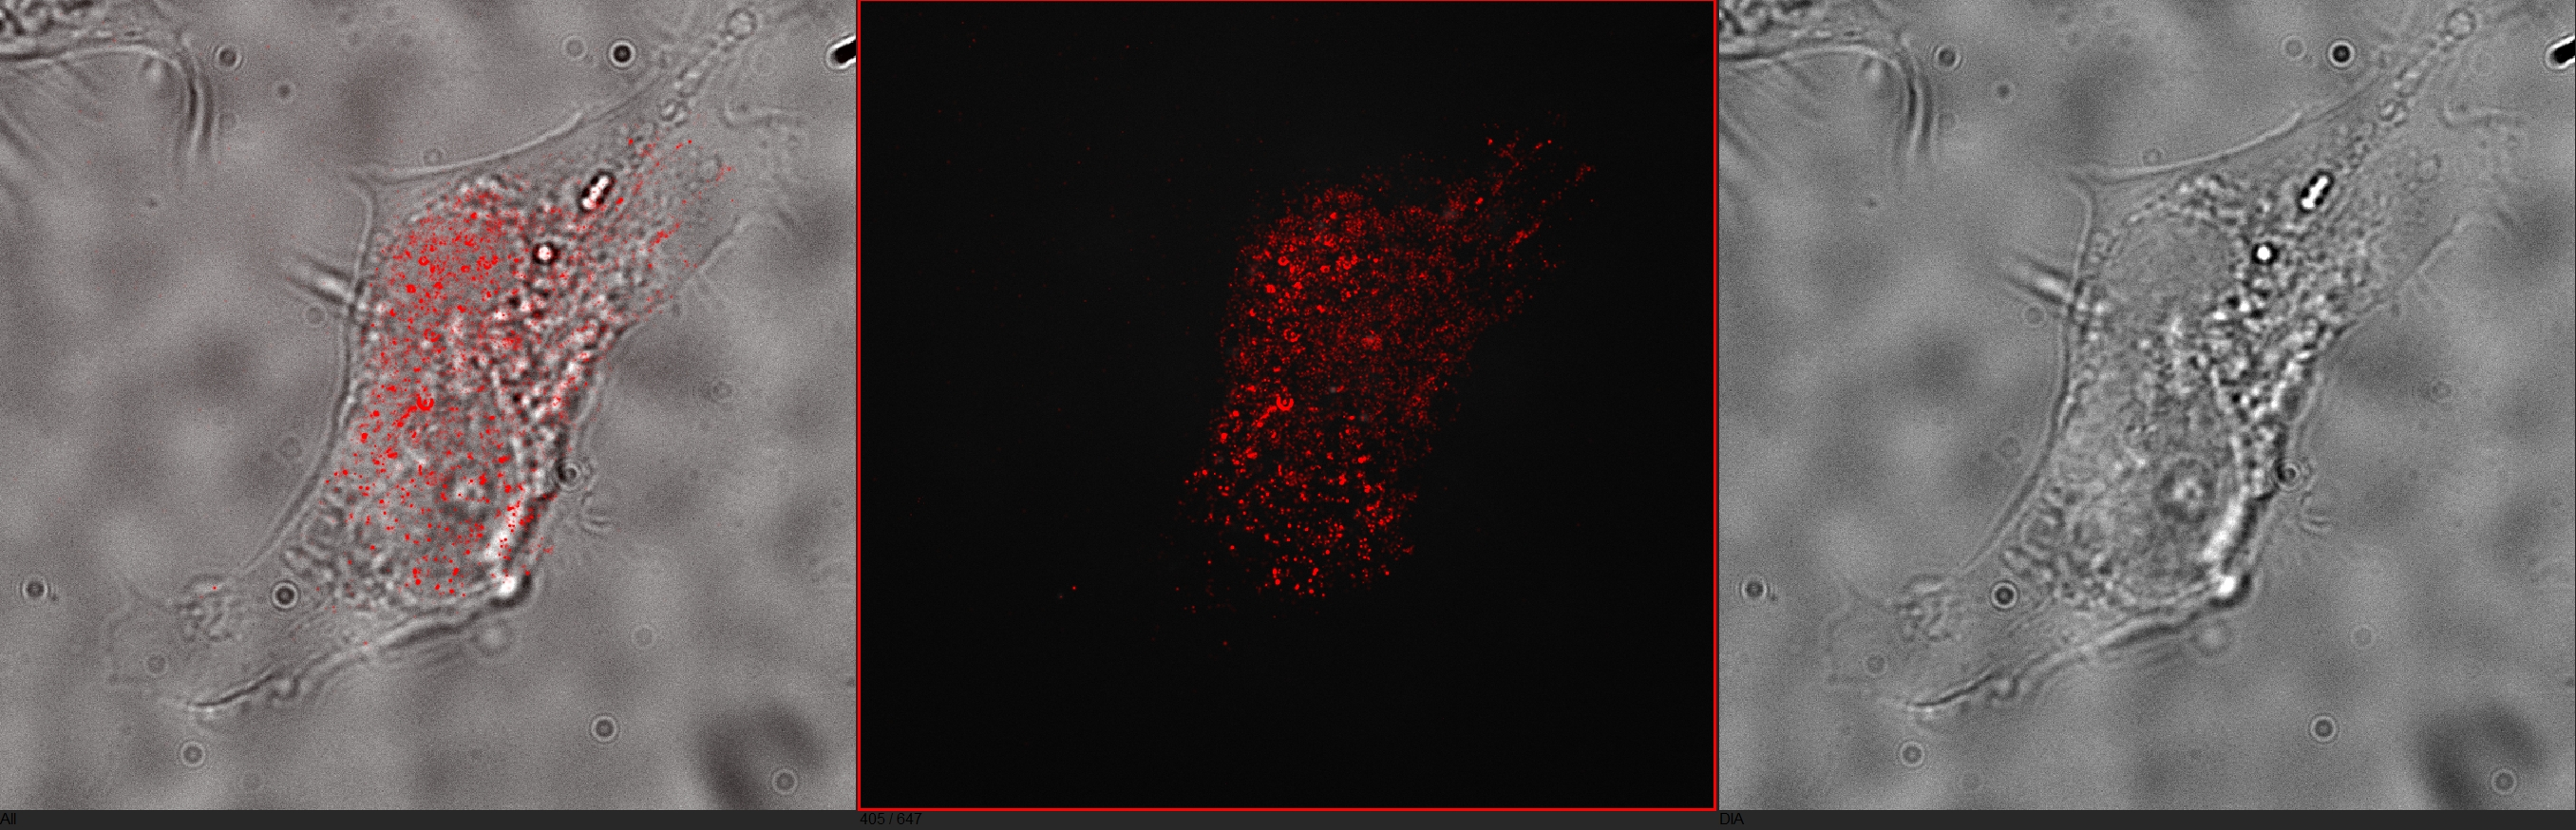
\includegraphics[width=3.4in]{Halo-tag PA646 - Fusion - 2x Mag - Area 1 - overlay.jpg}
\caption{\small \textbf{Modified protocol ensures intranuclear staining with PA-JF646, and heavily reduces non-specific, cytoplasmic binding.} From left to right, overlaid diascopic and fluorescence microscope images, only fluorescence image, only diascopic image. We see abundant nuclear signal, and that the cytoplasmic signal is reduced significantly. The fluorescence images were taken with a traditional photoactivatable localization microscopy (PALM) illumination scheme, but with the sole intention of verifying nuclear signal (i.e. with no intention of localization, the 405/647 nm beam powers were chosen arbitrarily).}
\label{fig1}
\hspace{1cm}
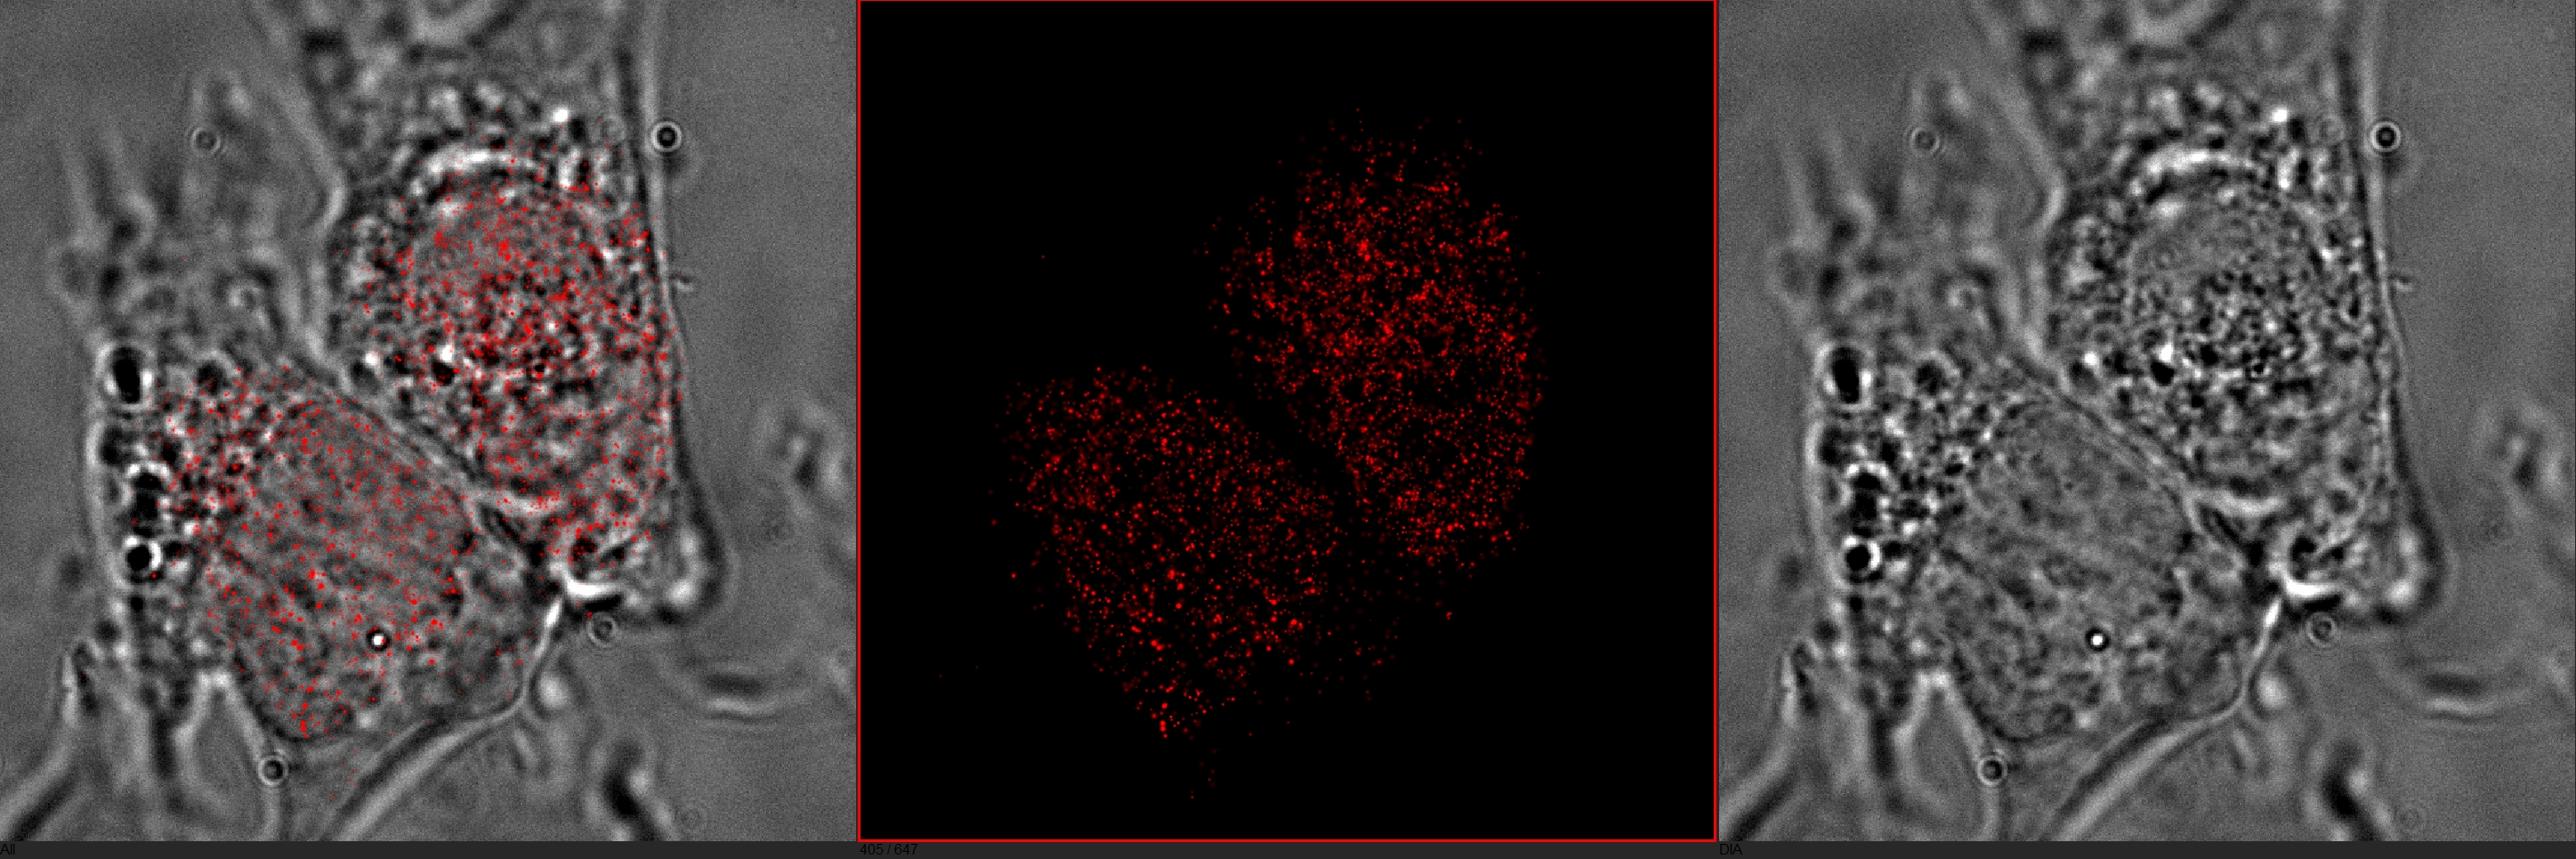
\includegraphics[width=3.4in]{Halo-tag PA549 - Fusion - 2x Mag - Area 4 - overlay.jpg}
\caption{\small \textbf{Modified protocol nearly eliminates non-specific, cytoplasmic binding of PA-JF549.} From left to right, overlaid diascopic and fluorescence microscope images, only fluorescence image, only diascopic image. The fluorescence images were taken with a traditional photoactivatable localization microscopy (PALM) illumination scheme, but with the sole intention of verifying nuclear signal (i.e. with no intention of localization, the 405/561 nm beam powers were chosen arbitrarily).}
\label{fig2}
\end{figure}

\end{document}

